\documentclass[border=10pt]{standalone}

\usepackage{tikz}
\usepackage{tikzsymbols}
\usetikzlibrary{calc,patterns,shapes.geometric}

\def\centerarc[#1](#2)(#3:#4:#5){\draw[#1] ($(#2)+({#5*cos(#3)},{#5*sin(#3)})$) arc (#3:#4:#5);}

\begin{document}
	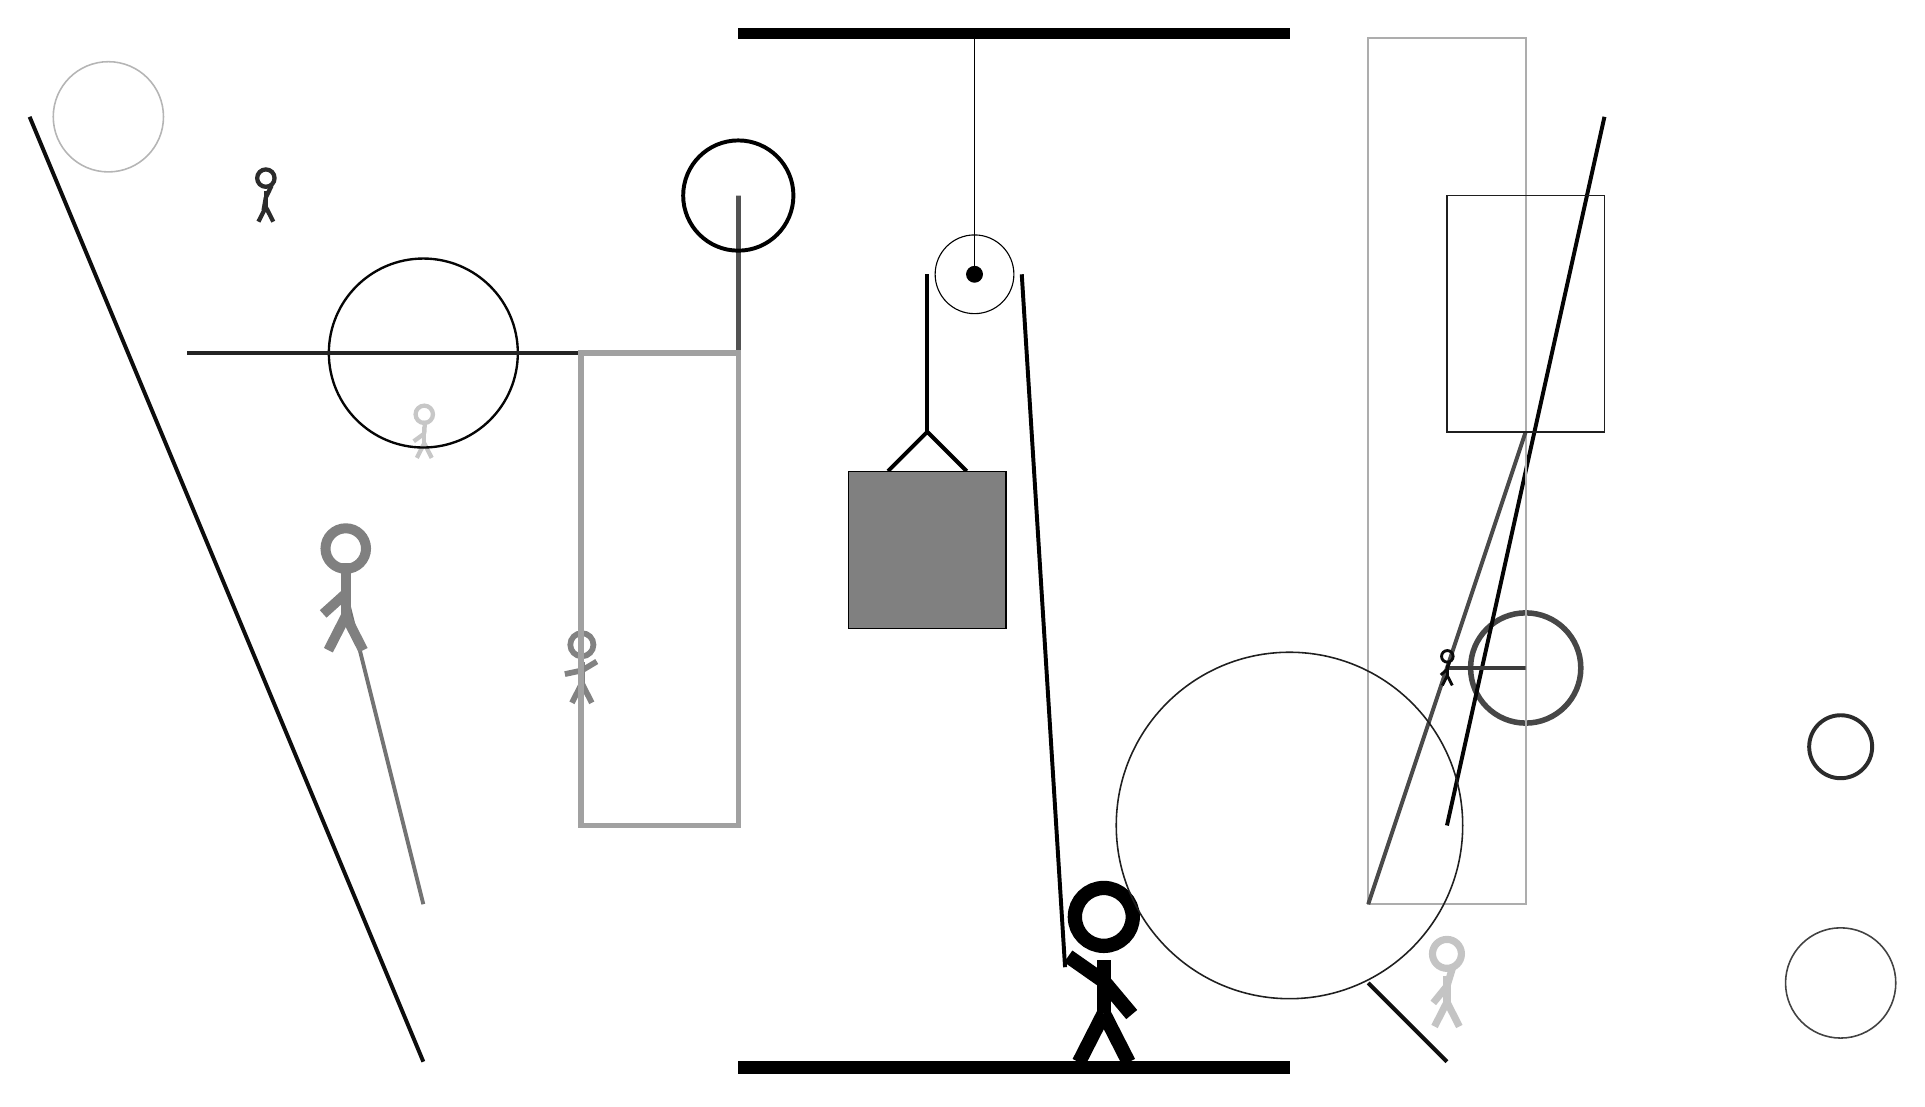
\begin{tikzpicture}
		%%%%% START %%%%%
		
		\draw[fill=black] (-2, 10) rectangle (5, 10.125);
		
		\draw (1, 7) circle (0.5);
		\draw[fill=black] (1, 7) circle (0.1);
		\draw (1, 10) -- (1, 7);
		
		\draw[line width=0.5mm] (-0.1, 4.5) -- (0.4, 5.0) -- (0.9, 4.5);
		\draw[fill=black!50] (-0.6, 4.5) rectangle (1.4, 2.5);
		
		\draw[line width=0.5mm] (0.4, 7) -- (0.4, 5.0);
		\centerarc[line width=0.5mm](1, 7)(0:180:0.6);
		\draw[line width=0.5mm](1.6, 7) -- (2.15, -1.8);
		
		\node at (2.6, -1.9) {\Strichmaxerl[10][-35][-50]};
		
		\draw [line width=0.7mm, color=black!72](8, 2) circle (0.7);
		
		\draw[line width=0.5mm, color=black!98](7, 0) -- (9, 9);
		\draw[line width=0.3mm, color=black!32] (6, -1) rectangle (8, 10);
		\node[line width=0.7mm, color=black!22] at (-6, 5) {\Strichmaxerl[3][36][87]};
		\draw [line width=0.2mm, color=black!29](-10, 9) circle (0.7);
		\draw[line width=0.5mm, color=black!95](-6, -3) -- (-11, 9);
		\draw[line width=0.5mm, color=black!71](6, -1) -- (8, 5);
		\draw[line width=0.5mm, color=black!55](-7, 3) -- (-6, -1);
		\draw [line width=0.3mm, color=black!98](-6, 6) circle (1.2);
		\draw [line width=0.5mm, color=black!83](12, 1) circle (0.4);
		\node[line width=0.7mm, color=black!50] at (-7, 3) {\Strichmaxerl[7][42][90]};
		\draw[line width=0.6mm, color=black!68] (-2, 8) rectangle (-2, 1);
		\draw[line width=0.6mm, color=black!77] (7, 2) rectangle (8, 2);
		\draw [line width=0.5mm, color=black!100](-2, 8) circle (0.7);
		\draw[line width=0.5mm, color=black!86](-2, 6) -- (-9, 6);
		\draw [line width=0.2mm, color=black!88](5, 0) circle (2.2);
		\node[line width=0.3mm, color=black!49] at (-4, 2) {\Strichmaxerl[4][12][31]};
		\draw[line width=0.5mm, color=black!94](7, -3) -- (6, -2);
		\draw [line width=0.2mm, color=black!74](12, -2) circle (0.7);
		\draw[line width=0.7mm, color=black!37] (-2, 6) rectangle (-4, 0);
		\draw[line width=0.2mm, color=black!88] (7, 8) rectangle (9, 5);
		
		\node[line width=0.2mm, color=black!23] at (7, -2) {\Strichmaxerl[5][51][73]};
		\node[line width=0.6mm, color=black!83] at (-8, 8) {\Strichmaxerl[3][80][64]};
		\node[line width=0.5mm, color=black!96] at (7, 2) {\Strichmaxerl[2][41][73]};
		
		\draw[fill=black] (-2, -3) rectangle (5, -3.15);
		
		%%%%% END %%%%%
	\end{tikzpicture}
\end{document}